\documentclass[12pt]{Homework}

% Changed from \usepackage{prelude}
\usepackage{preamble}
\usepackage{amssymb}
\usepackage{enumitem}
\usepackage{mathrsfs}
\def\upint{\mathchoice%
    {\mkern13mu\overline{\vphantom{\intop}\mkern7mu}\mkern-20mu}%
    {\mkern7mu\overline{\vphantom{\intop}\mkern7mu}\mkern-14mu}%
    {\mkern7mu\overline{\vphantom{\intop}\mkern7mu}\mkern-14mu}%
    {\mkern7mu\overline{\vphantom{\intop}\mkern7mu}\mkern-14mu}%
  \int}
\def\lowint{\mkern3mu\underline{\vphantom{\intop}\mkern7mu}\mkern-10mu\int}
\usepackage[mathscr]{euscript}
\usepackage{comment}
\usepackage{MnSymbol}
\usepackage{tikz,float}
\usepackage{tikz-cd}
\usepackage{graphicx}
\usepackage{mathtools}
\usepackage{bbding}
\renewcommand\qedsymbol{\Peace}
\newcommand\placeqed{\nobreak\enspace\Peace}
\usepackage{caption, threeparttable}
\usepackage{halloweenmath}
\newcommand{\contradiction}{\null\hfill\large{$\mathghost$}\normalsize}
\newcommand{\im}{\mathscr{I}\text{m}}
\newcommand{\re}{\mathscr{R}\text{e}}
\newcommand{\res}{\text{Res}}

\name{Kayla Orlinsky}
\course{Complex Analysis Exam}
\term{Fall 2010}
\hwnum{Fall 2010}

\begin{document}

\begin{problem} $\,$
Show that $$\int_0^\infty\frac{\sin x}{x(x^2+1)}dx=\frac{\pi(1-e^{-1})}{2}.$$
\end{problem}


\begin{solution}$\,$
We choose the countour below:

\begin{center}
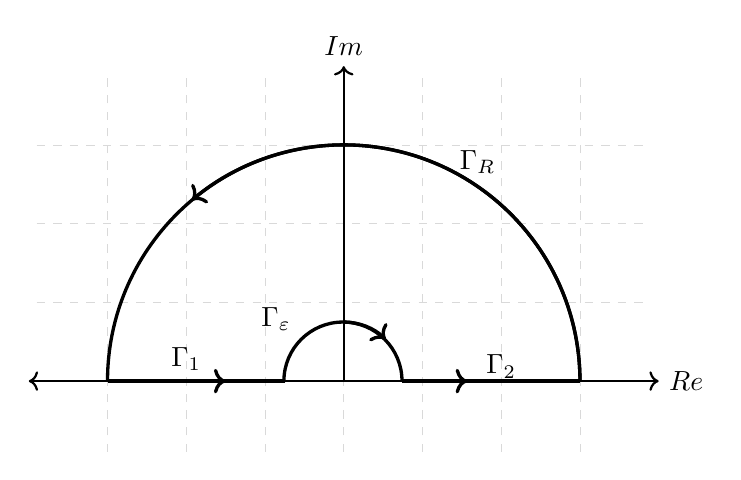
\begin{tikzpicture}
\draw[help lines, color=gray!30, dashed] (-3.9,-0.9) grid (3.9,3.9);
\draw[->,very thick] (3,0) arc (0:130:3cm);
\draw[very thick] (3,0) arc (0:180:3cm) node[above,yshift=2.5cm,xshift=4.7cm]{$\Gamma_R$};
\draw[->,very thick] (0,0.75) arc (90:45:0.75cm);
\draw[very thick] (0.74,0) arc (0:180:0.75cm) node[above,yshift=0.5cm,xshift=-0.1cm]{$\Gamma_\varepsilon$};
\draw[->,very thick] (0.74,0) -- (1.57,0);
\draw[very thick] (0.75,0) -- (3,0) node[above,yshift=-0.1cm,xshift=-1cm]{$\Gamma_2$};
\draw[->,very thick] (-3,0) -- (-1.5,0);
\draw[very thick] (-0.74,0) -- (-3,0) node[above,yshift=0cm,xshift=1cm]{$\Gamma_1$};
\draw[<->, thick] (-4,0)--(4,0) node[right]{$Re$};
\draw[->, thick] (0,0)--(0,4) node[above]{$Im$};
\end{tikzpicture}
\end{center}

Let \begin{align*}
    I_1&=\int_{\Gamma_1}\frac{e^{iz}}{z(z^2+1)}dz\\
    I_2&=\int_{\Gamma_2}\frac{e^{iz}}{z(z^2+1)}dz\\
    I_\varepsilon&=\int_{\Gamma_\varepsilon}\frac{e^{iz}}{z(z^2+1)}dz\\
    I_R&=\int_{\Gamma_R}\frac{e^{iz}}{z(z^2+1)}dz
\end{align*}

Then, we note that \begin{align*}
    I_1+I_2&=\int_{-R}^{-\varepsilon}\frac{e^{ix}}{x(x^2+1)}dx+\int_\varepsilon^R\frac{e^{ix}}{x(x^2+1)}dx\\
    &=\int_R^\varepsilon\frac{-e^{-iu}}{-u(u^2+1)}du+\int_\varepsilon^R\frac{e^{ix}}{x(x^2+1)}dx\qquad\text{plugging in }u=-x\\
    &=\int_\varepsilon^R\frac{-e^{ix}}{x(x^2+1)}dx+\int_\varepsilon^R\frac{e^{ix}}{x(x^2+1)}dx\qquad \text{plugging in }x=u\\
    &=\int_\varepsilon^R\frac{e^{ix}-e^{ix}}{x(x^2+1)}dx\\
    &=\int_\varepsilon^R\frac{2i\sin x}{x(x^2+1)}dx
\end{align*}

Now, \begin{align*}
    |I_R|&=\left|\int_{\Gamma_R}\frac{e^{iz}}{z(z^2+1)}dz\right|\\
    &\le\int_{|z|=R}\frac{|e^{iz}|}{|z||z^2+1|}|dz|\qquad \theta\in[0,\pi].\\
    &=\int_{|z|=R}\frac{e^{\Re(iRe^{i\theta})}}{R|z^2+1|}|dz|\qquad z=Re^{i\theta}\\
    &=\int_{|z|=R}\frac{e^{-R\sin\theta}}{R|z^2+1|}|dz|\\
    &\le\int_{|z|=R}\frac{e^{-R\sin\theta}}{R^3}|dz|\\
    &\le \int_{|z|=R}\frac{1}{R^3}|dz|\\
    &=\frac{2\pi R}{R^3}\\
    &=\frac{2\pi}{R^2}\to0\text{ as }R\to\infty
\end{align*}

since $\sin\theta$ is non-negative on the upper half circle and so $e^{-R\sin\theta}\le1$ for $R$ large.  

Now, for $I_\varepsilon,$ we note that $\frac{e^{iz}}{z(z^2+1)}$ has an isolated pole of order $1$ at $0$, and so, for $\varepsilon$ small, we have that $\frac{e^{iz}}{z(z^2+1)}=\frac{a}{z}+f(z)$ for $f(z)$ analytic at $0$ and $$a=\res_{z=0}\frac{e^{iz}}{z(z^2+1)}=\frac{e^{0}}{1}=1$$ is the reside of $\frac{e^{iz}}{z(z^2+1)}$ at $z=0.$

Therefore, \begin{align*}
    I_\varepsilon&=\int_{\Gamma_\varepsilon}\frac{e^{iz}}{z(z^2+1)}dz\\
    &=\int_{\Gamma_\varepsilon}\frac{1}{z}+f(z)dz\\
    &=\int_\pi^0i+i\varepsilon e^{i\theta}f(\varepsilon e^{i\theta})d\theta\\
    &=-\pi i+\int_\pi^0i\varepsilon e^{i\theta}f(\varepsilon e^{i\theta})d\theta\to-\pi i\qquad\varepsilon\to0
\end{align*}  since $f$ is analytic so $$\lim_{\varepsilon\to0}\int_\pi^0i\varepsilon e^{i\theta}f(\varepsilon e^{i\theta})d\theta=\int_\pi^0\lim_{\varepsilon\to0}i\varepsilon e^{i\theta}f(\varepsilon e^{i\theta})d\theta=0.$$

Finally, \begin{align*}
    \int_0^\infty\frac{2i\sin x}{x(x^2+1)}dx-\pi i&=\lim_{R\to\infty}\lim_{\varepsilon\to 0}(I_1+I_2+I_\varepsilon+I_R)\\
    &=2\pi i \res_{z=i}\frac{e^{iz}}{z(z^2+1)}\\
    &=2\pi i\frac{e^{i\cdot i}}{i(i+i)}\\
    &=\pi \frac{e^{-1}}{i}\\
    &=-\pi i e^{-1}
    \implies 2i\int_0^\infty\frac{\sin x}{x(x^2+1)}dx&=\pi i-\pi ie^{-1}\\
    \int_0^\infty\frac{\sin x}{x(x^2+1)}dx&=\frac{\pi i(1-e^{-1})}{2i}=\frac{\pi(1-e^{-1}}{2}
\end{align*}
\end{solution}
\newpage

\begin{problem} $\,$
Suppose that $f$ is holomorphic in a neighborhood of $0$ and that \begin{align*}
    \sum_{n=0}^\infty f^{(n)}(z) \tag{1}
\end{align*} is absolutely convergent at $z=0$. Show that $f$ is an entire function and that (1) is convergent for all $z\in\mathbb{C}$.
\end{problem}


\begin{solution}$\,$
Note that the Taylor expansion for $f$ is $$f(z)=\sum_{n=0}^\infty f^{(n)}(0)\frac{z^n}{n!}.$$ $f$ is anlalytic at $z$ if and only if the Taylor expansion for $f$ is absolutely convergent at $z.$

Thus, we will show that the Taylor expansion is uniformly convergent so $f$ is entire. However, this is immediate since $$\left|\sum_{n=0}^\infty f^{(n)}(0)\frac{z^n}{n!}\right|\le\left(\sum_{n=0}^\infty|f^{(n)}(0)|\right)\left(\sum_{n=0}^\infty\frac{|z|^n}{n!}\right)=e^{|z|}\sum_{n=0}^\infty|f^{(n)}(0)|<\infty$$ for all $z$ since $e^z$ is analytic and finite for each fixed $z$ and $\sum_{n=0}^\infty|f^{(n)}(0)|$ is finite.

Therefore, the partial sums of the Taylor series for $f$ are bounded by a constant times the partial sums of the Taylor series for $e^z$ (which is entire and so has uniformly convergent Taylor series) for each $z$ the sum is absolutely convergent and so $f$ is entire. Now, \begin{align*}
    \left|\sum_{n=0}^\infty f^{(n)}(z)\right|&=\left|\sum_{n=0}^\infty\sum_{k=n}^\infty f^{(k)}(0)\frac{z^{k-n}}{(k-n)1}\right|\\
    &=\left|\sum_{k=0}^\infty f^{(k)}(0)\frac{z^k}{k!}+\sum_{k=1}^\infty f^{(k)}(0)\frac{z^{k-1}}{(k-1)!}+\sum_{k=2}^\infty f^{(k)}(0)\frac{z^{k-2}}{(k-2)!}+\cdots\right|\\
    &=\begin{vmatrix}
    f^{(0)}(0) & + f^{(1)}(0)z & + f^{(2)}(0)\frac{z^2}{2!} & + f^{(3)}(0)\frac{z^3}{3!} &+\cdots\\
    & + f^{(1)}(0) & + f^{(2)}(0)z & + f^{(3)}(0)\frac{z^2}{2!} & +\cdots\\
    & & +f^{(2)}(0) & + f^{(3)}(0)z &+\cdots \\
    & & & + f^{(3)}(0) & +\cdots
    \end{vmatrix}\\
    &=\left|\sum_{k=0}^\infty\sum_{n=0}^kf^{(k)}(0)\frac{z^{k-n}}{(k-n)!}\right|\\
    &=\left|\sum_{k=0}^\infty f^{(k)}(0)\sum_{n=0}^k\frac{z^{k-n}}{(k-n)!}\right|\\
    &\le \sum_{k=0}^\infty|f^{(k)}(0)|\sum_{n=0}^k\left|\frac{z^{k-n}}{(k-n)!}\right|\\
    &\le M e^{|z|}
\end{align*}

and again, since $e^z$ is finite for all fixed $z$, we have that the sum converges absolutely.
\end{solution}
\newpage

\begin{problem} $\,$
Let $f$ be a non-negative real valued harmonic function in the disc $D=\{z\in\mathbb{C}:|z|<R\}.$
\begin{enumerate}[label=(\alph*)]
    \item Prove that $$\frac{R-|z|}{R+|z|}f(0)\le f(z)\le\frac{R+|z|}{R-|z|}f(0)\qquad\text{whenever }|z|<R.$$ Hint: use the Poisson formula.
    \item Prove that $$\frac{1}{3}f(0)\le f(z)\le 3f(0)\qquad\text{whenever }|z|\le R/2.$$
    \item Let $K$ be a compact subset of the open disc $D.$ Show that there is a constant $M$ depending only on $K$ and $R$ such that $$f(z_1)\le Mf(z_2)\qquad\text{ for all }z_1,z_2\in K.$$
\end{enumerate}
\end{problem}


\begin{solution}$\,$
\begin{enumerate}[label=(\alph*)]
    \item Since $f$ is harmonic on a disk of radius $R$ we can apply the Poisson Formula to obtain $$f(z)=\frac{1}{2\pi}\int_{|\xi|=R}\frac{R^2-|z|^2}{|\xi-z|^2}f(\xi)d\theta$$ and since $$(R-|z|)^2\le|\xi-z|^2\le(R+|z|)^2$$ and since $f$ is non-negative so $f(\xi)\ge0$ for all $\xi$, we can write $$ \frac{1}{2\pi}\int_{|\xi|=R}\frac{R^2-|z|^2}{(R+|z|)^2}f(\xi)d\theta\le \frac{1}{2\pi}\int_{|\xi|=R}\frac{R^2-|z|^2}{|\xi-z|^2}f(\xi)d\theta\le f(z)$$ and $$f(z)\le \frac{1}{2\pi}\int_{|\xi|=R}\frac{R^2-|z|^2}{|\xi-z|^2}f(\xi)d\theta\le \frac{1}{2\pi}\int_{|\xi|=R}\frac{R^2-|z|^2}{(R-|z|)^2}f(\xi)d\theta$$ so \begin{align*}
        \frac{1}{2\pi}\int_{|\xi|=R}\frac{R-|z|}{R+|z|}f(\xi)d\theta\le &f(z)\le  \frac{1}{2\pi}\int_{|\xi|=R}\frac{R+|z|}{R-|z|}f(\xi)d\theta\\
        \frac{R-|z|}{R+|z|}\frac{1}{2\pi}\int_{|\xi|=R}f(\xi)d\theta\le &f(z)\le \frac{R+|z|}{R-|z|}\frac{1}{2\pi}\int_{|\xi|=R}f(\xi)d\theta\\
        \frac{R-|z|}{R+|z|}f(0)\le &f(z)\le \frac{R+|z|}{R-|z|} f(0)
    \end{align*}
    \item Since $$R-|z|\ge R-R/2=R/2$$ and $$R+|z|\le R+R/2=3R/2$$ we get that $$\frac{R-|z|}{R+|z|}\ge \frac{R/2}{3R/2}=\frac{1}{3}$$ and $$\frac{R+|z|}{R-|z|}\le \frac{3R/2}{R/2}=3$$
    
    so applying (a), we obtain the result $$\frac{1}{3}f(0)\le f(z)\le 3f(0)\qquad\text{whenever }|z|\le R/2.$$
    \item Because $K\subset D=\{z\,|\,|z|<R\}$, we have that there exists an $r<R$ such that $K\subset E=\{z\,|\,  |z|\le r\}.$
    
    Therefore, if $z_1,z_2\in K$, then $z_1,z_2\in E$ and so \begin{align*}
        \frac{R-|z_2|}{R+|z_2|}f(0)\le & f(z_2)\\
        & f(z_1)\le \frac{R+|z_1|}{R-|z_2|}f(0)\\
       f(z_1)\frac{R-|z_1|}{R+|z_1|} \le &f(0)\le f(z_2)\frac{R+|z_2|}{R-|z_2|}\\
       f(z_1)&\le \frac{(R+|z_1|)(R+|z_2|)}{(R-|z_1|)(R-|z_2|)}
    \end{align*}
\end{enumerate}
\end{solution}
\newpage





\begin{problem} $\,$ Liouville's theorem states that a bounded entire function $f$ is constant.
\begin{enumerate}[label=(\alph*)]
    \item Give a proof of Liouville's theorem. You may use standard results about holomorphic functions such as Cauchy's theorem and power series representation, but any result you use should be clearly stated.
    \item Suppose instead that $f$ is entire and that $|f(z)|\le K(1+|z|^n)$ for some $K<\infty$ and positive integer $n.$ Show that $f$ is a polynomial of degree at most $n.$
\end{enumerate}
\end{problem}


\begin{solution}$\,$
\begin{enumerate}[label=(\alph*)]
    \item Assume $f$ is entire and bounded. Say $|f(z)|\le M$ for all $z.$
    
    Then, for any $R>0$, by Cauchy, \begin{align*}
        |f'(z)|&=\left|\frac{1}{2\pi i}\int_{|\zeta|=R}\frac{f(\zeta)}{(\zeta-z)^2}d\zeta\right|\\
        &\le \frac{1}{2\pi}\int_{|\zeta|=R}\frac{M}{|\zeta-z|^2}|d\zeta|\\
        &=M\frac{1}{2\pi}\int_0^{2\pi}\frac{1}{R}d\theta \qquad \begin{matrix}
        \zeta= z+Re^{i\theta}\\
        d\zeta = Rie^{i\theta}d\theta
        \end{matrix}\\
        &=\frac{M}{R}
    \end{align*} and since $R$ is arbitrary, taking $R\to\infty$ we get that $|f'(z)|=0$ for all $z$ and so $f$ is constant.
    \item Since $f$ is entire, it has a well defined Taylor series at $0$, namely, $$f(z)=\sum_{n=0}^\infty f^{(n)}(a)\frac{(z-a)^n}{n!}\qquad\text{ for all }z.$$
    
    We will use a similar argument as before, namely, \begin{align*}
        |f^{(n+1)}(z)|&=\left|\frac{(n+1)!}{2\pi i}\int_{|\zeta|=R}\frac{f(\zeta)}{(\zeta-z)^{n+2}}d\zeta\right|\\
        &\le \frac{(n+1)!}{2\pi}\int_{|\zeta|=R}\frac{K(1+|z|^n)}{|\zeta-z|^2}|d\zeta|\\
        &=K\frac{(n+1)!}{2\pi}\int_0^{2\pi}\frac{1+|z|^n}{R^{n+1}}d\theta\\
        &=K(n+1)!\frac{1+|z|^n}{R^{n+1}}\\
        &\le K(n+1)!\frac{1+R^n}{R^{n+1}}    
    \end{align*}
    
    and since this tends to $0$ as $R\to\infty$, again we conclude that $f^{(n+1)}(z)=0$ for all $z$, and so every Taylor series for $f$ dies after at most $n$ terms.
    
    Namely, $f$ is a polynomial of degree at most $n.$
\end{enumerate}
\end{solution}


\end{document}
 